\documentclass[tikz,border=3pt]{standalone}
\usepackage{amsmath,amssymb}
\usetikzlibrary{decorations.pathmorphing,decorations.pathreplacing,patterns,arrows.meta,shapes.geometric,calc,positioning}

% colour-blind-safe palette
\definecolor{emit}{HTML}{0072B2}   % blue: emissions / forward
\definecolor{dark}{HTML}{D55E00}   % vermilion: dark counts
\definecolor{dead}{HTML}{BBBBBB}   % grey: dead bins
\definecolor{bad}{HTML}{CC0000}

\tikzset{
  lbl/.style={font=\small},
  small/.style={font=\footnotesize},
  anc/.style={circle,draw=black!70,fill=black!6,minimum size=3.2mm,inner sep=0},
  ancx/.style={circle,draw=emit,fill=emit,minimum size=3.2mm,inner sep=0},
  phot/.style={circle,fill=emit,minimum size=2.2mm,inner sep=0},
  miss/.style={circle,draw=emit,thick,fill=white,minimum size=2.2mm,inner sep=0},
  dc/.style={star,star points=5,star point ratio=2.2,fill=dark,minimum size=3mm,inner sep=0},
  panel/.style={font=\bfseries\normalsize},
}

\begin{document}
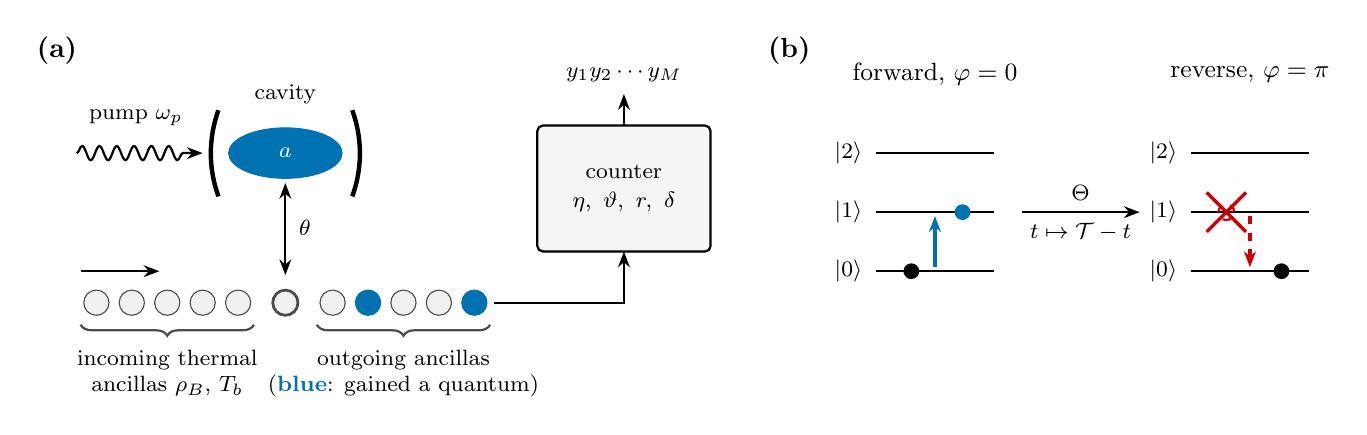
\begin{tikzpicture}[>={Stealth[length=2mm]}]

%==================== (a) setup ====================
\node[panel] at (0,4.3) {(a)};

% pump
\draw[->,thick,decorate,decoration={snake,amplitude=0.9mm,segment length=2.2mm,post length=2mm}]
  (0.25,3.0) -- (1.85,3.0);
\node[small] at (1.0,3.45) {pump $\omega_p$};

% cavity mirrors
\draw[line width=1.6pt] (2.05,2.45) arc[start angle=200,end angle=160,radius=1.6];
\draw[line width=1.6pt] (3.75,2.45) arc[start angle=-20,end angle=20,radius=1.6];
\draw[emit,fill=emit] (2.9,3.0) ellipse (0.72 and 0.32);
\node[small,text=white] at (2.9,3.0) {$a$};
\node[small] at (2.9,3.75) {cavity};

% coupling to ancilla stream
\draw[<->,thick] (2.9,2.62) -- (2.9,1.45);
\node[small,anchor=west] at (2.95,2.05) {$\theta$};

% ancilla stream
\foreach \x in {0.5,0.95,1.4,1.85,2.3} \node[anc] at (\x,1.1) {};
\node[anc,line width=1pt] at (2.9,1.1) {};
\foreach \x/\s in {3.5/anc,3.95/ancx,4.4/anc,4.85/anc,5.3/ancx}
  \node[\s] at (\x,1.1) {};
\draw[decorate,decoration={brace,mirror,amplitude=4pt},thick,black!70] (0.3,0.82) -- (2.5,0.82);
\node[small,align=center,anchor=north] at (1.4,0.62) {incoming thermal\\ancillas $\rho_B$, $T_b$};
\draw[decorate,decoration={brace,mirror,amplitude=4pt},thick,black!70] (3.3,0.82) -- (5.5,0.82);
\node[small,align=center,anchor=north] at (4.4,0.62) {outgoing ancillas\\(\textcolor{emit}{\textbf{blue}}: gained a quantum)};
\draw[->,thick,black] (0.3,1.5) -- (1.3,1.5);

% counter
\draw[rounded corners=2pt,thick,fill=black!4] (6.1,1.75) rectangle (8.3,3.35);
\node[small,align=center] at (7.2,2.55) {counter\\[1pt]$\eta,\ \vartheta,\ r,\ \delta$};
\draw[->,thick] (5.55,1.1) -| (7.2,1.75);
\draw[->,thick] (7.2,3.35) -- (7.2,3.75);
\node[small] at (7.2,4.0) {$y_1y_2\cdots y_M$};

%==================== (b) forward vs reverse ====================
\begin{scope}[xshift=9.3cm]
\node[panel] at (0,4.3) {(b)};

% ---- forward ----
\node[lbl] at (1.85,4.0) {forward, $\varphi=0$};
\foreach \k in {0,1,2} {
  \draw[thick] (1.1,1.5+0.75*\k) -- (2.6,1.5+0.75*\k);
  \node[small,anchor=east] at (1.05,1.5+0.75*\k) {$|\k\rangle$};
}
\node[circle,fill=black,minimum size=2mm,inner sep=0] at (1.55,1.5) {};
\draw[->,very thick,emit] (1.85,1.55) -- (1.85,2.2);
\node[circle,fill=emit,minimum size=2mm,inner sep=0] at (2.2,2.25) {};

% ---- alignment arrow ----
\draw[->,thick,black] (2.95,2.25) -- (4.45,2.25);
\node[small] at (3.7,2.5) {$\Theta$};
\node[small] at (3.7,2.0) {$t\mapsto\mathcal T-t$};

% ---- reverse ----
\node[lbl] at (5.85,4.0) {reverse, $\varphi=\pi$};
\foreach \k in {0,1,2} {
  \draw[thick] (5.1,1.5+0.75*\k) -- (6.6,1.5+0.75*\k);
  \node[small,anchor=east] at (5.05,1.5+0.75*\k) {$|\k\rangle$};
}
\node[circle,draw=bad,dashed,thick,minimum size=2mm,inner sep=0] at (5.55,2.25) {};
\draw[->,very thick,bad,dashed] (5.85,2.2) -- (5.85,1.55);
\node[circle,fill=black,minimum size=2mm,inner sep=0] at (6.25,1.5) {};
\draw[bad,very thick] (5.3,2.0) -- (5.8,2.5) (5.3,2.5) -- (5.8,2.0);

\end{scope}

\end{tikzpicture}
\end{document}
